\documentclass[
	% -- opções da classe memoir --
	article,			% indica que é um artigo acadêmico
	12pt,				% tamanho da fonte
	oneside,			% para impressão apenas no recto. Oposto a twoside
	a4paper,			% tamanho do papel.
	% -- opções da classe abntex2 --
	%chapter=TITLE,		% títulos de capítulos convertidos em letras maiúsculas
	%section=TITLE,		% títulos de seções convertidos em letras maiúsculas
	%subsection=TITLE,	% títulos de subseções convertidos em letras maiúsculas
	%subsubsection=TITLE % títulos de subsubseções convertidos em letras maiúsculas
	% -- opções do pacote babel --
	english,			% idioma adicional para hifenização
	brazil,				% o último idioma é o principal do documento
	sumario=tradicional
	]{abntex2}


% ---
% PACOTES
% ---

\usepackage{lmodern}			% Usa a fonte Latin Modern
\usepackage[T1]{fontenc}		% Selecao de codigos de fonte.
\usepackage[utf8]{inputenc}		% Codificacao do documento (conversão automática dos acentos)
\usepackage{indentfirst}		% Indenta o primeiro parágrafo de cada seção.
\usepackage{nomencl} 			% Lista de simbolos
\usepackage{color}				% Controle das cores
\usepackage{graphicx}			% Inclusão de gráficos
\usepackage{microtype} 			% para melhorias de justificação
% ---

% ---
% Pacotes de citações
% ---
\usepackage[brazilian,hyperpageref]{backref}	 % Paginas com as citações na bibl
\usepackage[alf]{abntex2cite}	% Citações padrão ABNT
% ---

% ---
% Configurações do pacote backref
% Usado sem a opção hyperpageref de backref
\renewcommand{\backrefpagesname}{Citado na(s) página(s):~}
% Texto padrão antes do número das páginas
\renewcommand{\backref}{}
% Define os textos da citação
\renewcommand*{\backrefalt}[4]{
	\ifcase #1 %
		Nenhuma citação no texto.%
	\or
		Citado na página #2.%
	\else
		Citado #1 vezes nas páginas #2.%
	\fi}%
% ---

% ---
% Informações de dados para CAPA e FOLHA DE ROSTO
% ---
\titulo{Criptografia Simétrica D.E.S - Data Encryption Standard}
\autor{Angelo Rodrigo Ribeiro da Silva\thanks{angelorodriigo.rs@gmail.com} Jaíne da Silva Santos\thanks{jaine.ssilva1@gmail.com}
\\Jonatas Rosa da Silva Bonventi\thanks{jonatasbvt@yahoo.com} Dante Mesquita Neto\thanks{dantemesquitaneto@gmail.com}}
\local{Brasil}
\data{2017}

% Configurações de aparência do PDF final

% alterando o aspecto da cor azul
\definecolor{blue}{RGB}{41,5,195}

% informações do PDF
\makeatletter
\hypersetup{
     	%pagebackref=true,
		pdftitle={\@title},
		pdfauthor={\@author},
    	pdfsubject={Criptografia Simétrica D.E.S - Data Encryption Standard},
	    pdfcreator={LaTeX with abnTeX2},
		pdfkeywords={des}{Data Encryption Standard}{criptografia}{segurança da informação}{ifsp},
		colorlinks=true,       		% false: boxed links; true: colored links
    	linkcolor=blue,          	% color of internal links
    	citecolor=blue,        		% color of links to bibliography
    	filecolor=magenta,      		% color of file links
		urlcolor=blue,
		bookmarksdepth=4
}
\makeatother


% compila o indice
\makeindex

% Margens segundo abnt
\setlrmarginsandblock{3cm}{3cm}{*}
\setulmarginsandblock{3cm}{3cm}{*}
\checkandfixthelayout

% ---
% Espaçamentos entre linhas e parágrafos
% ---

% O tamanho do parágrafo é dado por:
\setlength{\parindent}{1.3cm}

% Controle do espaçamento entre um parágrafo e outro:
\setlength{\parskip}{0.2cm}  % tente também \onelineskip

% Espaçamento simples
\SingleSpacing

% Início do documento
\begin{document}

% Seleciona o idioma do documento (conforme pacotes do babel)
\selectlanguage{brazil}

% Retira espaço extra obsoleto entre as frases.
\frenchspacing

% ELEMENTOS PRÉ-TEXTUAIS
% página de titulo
\maketitle

% resumo em português
\begin{resumoumacoluna}
 Resumo de uma coluna.

 \vspace{\onelineskip}

 \noindent
 \textbf{Palavras-chave}: des. Data Encryption Standard. criptografia. ifsp.
\end{resumoumacoluna}

% ELEMENTOS TEXTUAIS
\textual

% Introdução
\section*{Introdução}
\addcontentsline{toc}{section}{Introdução}
\nocite{sistema-des}
\nocite{criptografia-simetrica-assimetrica-cifragem}
\nocite{estudo-descritivo-criptografia}

A evolução das empresas de tecnologia, trouxe o advento da informação como patrimônio, portanto, é imprescindível alocação de recursos para protegê-la.

A metodologia utilizada para proteção dos dados dos sistemas de informação é a criptografia, que possui muitas implementações e algoritmos diferentes para a codificação dos dados.

Durante este artigo iremos introduzir o algoritmo DES (Data Encryption Standard), que utiliza o modelo de criptografia simétrica, ele é amplamente conhecido e utilizado em sistemas de comunicações.

\section{Criptografia Simétrica}

A criptografia simétrica é o modelo mais antigo de criptografia. Nos algoritmos de criptografia simétrica, o receptor e o emissor precisam conhecer a chave que será utilizada, para que os dois possam visualizar a mensagem.

A criptografia simétrica, também conhecida como criptografia de chave privada, se faz uma opção muito segura na comunicação, onde mesmo se um terceiro (invasor), conhecer a mensagem criptografada e o algoritmo, não irá conseguir visualizar a mensagem, pois não possui a chave de criptografia.

\section{Data Encryption Standard}

O DES (Data Encryption Standard) é um algoritmo simétrico que utiliza um tamanho de 64 bits. Para cada 64 bits de texto plano, gera 64 bits de texto criptografado, o faz, dividindo a mensagem em vários blocos, a preparando para o algoritmo de criptografia.

Sua chave possui um tamanho de 64 bits, sendo utilizados somente 56, pois 8 bits são reservados para paridade.

Na cifra DES, utilizamos para a criptografia uma série de permutações e substituições. Cada bloco do DES, utiliza uma substituição e uma permutação, o DES possui 16 destes blocos. Utilizando apenas operações aritméticas e lógicas, facilitou muito seu uso em hardware.

Atualmente, o DES foi substituido, entrando em seu lugar o Advanced Encryption Standard (AES), ele foi trocado principalmente pela sua insegurança ao utilizar uma chave de apenas 56 bits. O DES já conseguiu, através de alguns algoritmos ter sua chave quebrada em menos de 24 horas.


\subsection{Pré Criptografia Opcional}

Para realizar os ciclos de criptografia do DES, é muito recomendado que convertamos os dados para números e então binários, para que possamos melhorar tanto a segurança quanto a performance da cifra, a baixo temos um exemplo:

\begin{table}[h]
\centering
\caption{Tabela de substituição}
\label{my-label}
\begin{tabular}{|l|l|l|l|l|l|l|l|l|l|l|l|l|l|l|l|l|l|l|}
\hline
A  & B  & C  & D  & E  & F  & G  & H  & I  & J  & K  & L  & M  & N  & O  & P  & Q  & R  & S  \\ \hline
15 & 16 & 17 & 18 & 19 & 20 & 21 & 22 & 23 & 24 & 25 & 26 & 27 & 28 & 29 & 30 & 31 & 32 & 33 \\ \hline
\end{tabular}

\begin{tabular}{|l|l|l|l|l|l|l|l|l|l|l|l|l|l|l|l|}
\hline
T  & U  & V  & X  & Y  & Z  & 1  & 2  & 3  & 4  & 5  & 6  & 7  & 8  & 9  & - \\ \hline
34 & 35 & 36 & 37 & 38 & 39 & 40 & 41 & 42 & 43 & 44 & 45 & 46 & 47 & 48 & 49 \\ \hline
\end{tabular}
\end{table}

Utilizando a tabela, subtituímos as letras pelos números, ignorando os acentos e letras maíusculas. O número 49 irá ser utilizado para substituir os espaços.

O uso de 2 digitos para representar cada letra, evita a ambiguidade. Por exemplo, se a letra A fosse representada pelo número 3 e a letra B pelo número 4, logo "AB" seria representado por 34, porém o número 7 também seria representado por 34.

\subsection{Como o DES criptografa uma mensagem?}

Imagine que temos um texto simples de 64 bit. Essa mensagem vai ser colocada (input) num bloco de cifra do DES que vai mostrar (output) uma mensagem criptografada. A decriptação vai ser realizada utilizando o mesmo algoritmo da encriptação, trocando apenas as ordens das chaves. Veja:\\

\begin{figure}[!htb]
	\centering
	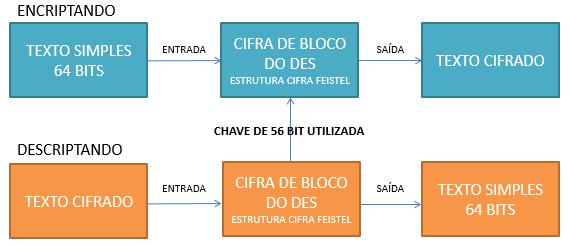
\includegraphics{encriptando_descriptando}
	\caption{Encriptando e descriptando com DES}
	\label{encriptando_descriptando_des}
\end{figure}

\subsection{Fluxo do algoritmo}

O esquema geral para criptografia DES está ilustrado na figura abaixo.

\begin{figure}[!htb]
	\centering
	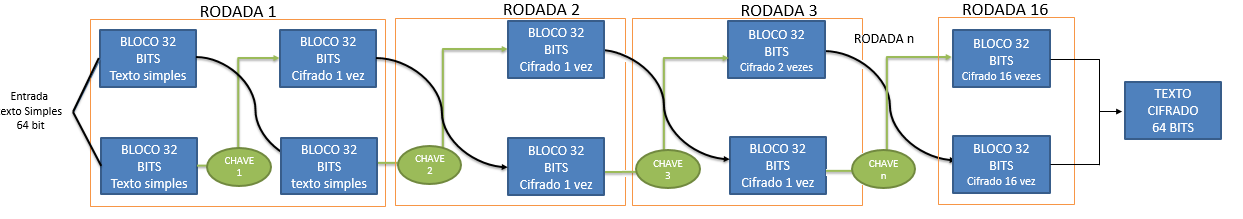
\includegraphics[scale=0.5]{esquema_geral}
	\caption{Encriptando com DES.}
	\label{esquema_geral_des}
\end{figure}

Assim como em qualquer esquema de criptografia, existem duas entradas na função de criptografia: O texto claro a ser codificado e a chave. Nesse caso, o texto precisa ter 64 bits de extensão e a chave tem 56 bits de extensão (na realidade, a função espera uma chave de 64 bits como entrada. Porém, somente 56 desses bits serão utilizados; os outros 8 bits podem ser usados como bits de paridade ou simplesmente definidos arbitrariamente).

Examinando de baixo da figura, podemos ver que o processamento do texto claro prossegue em três fases. Primeiro, o texto claro de 64 bits passa por uma permutação inicial, que reorganiza os bits para produzir a entrada permutada. Isso é seguido por uma fase consistindo em 16 rodadas da mesma função, que envolvem funções de permutação e substituição. A saída da última (décima sexta) rodada consiste em 64 bits que são uma função do texto claro de entrada e da chave. As metades da esquerda e da direita e da saída são trocadas para produzir a pré-saída. Finalmente, a pré-saída é passada por uma permutação (IP-¹) que é o inverso da função de permutação inicial (ou seja, ele executa o mesmo algoritmo, porém, executando da última chave para a primeira), o DES tem a estrutura exata e uma cifra de Feistel.

A chave de 56 bits é utilizada da seguinte forma: Inicialmente, a chave é passada por uma função de permutação. Depois, para cada uma das 16 rodadas, uma subchave é produzida pela combinação de um deslocamento circular à esquerda e uma permutação. A função de permutação é a mesma para cada rodada, mas uma subchave diferente é produzida, devido aos deslocamentos repetidos dos bits da chave.

Permutação inicial - A permutação inicial e seu inverso são definidos por tabelas, como mostram as tabelas abaixo, respectivamente. As tabelas devem ser interpretadas da seguinte maneira. A entrada de uma tabela consiste em 64 bits numerados de 1 a 64. As 64 entradas na tabela de permutação contêm uma permutação dos números de 1 a 64. Cada entrada na tabela de permutação indica a posição de um bit de entrada numerado na saída, que também consiste em 64 bits. Para ver que essas duas funções de permutação são realmente o inverso uma da outra, considere a seguinte entrada M de 64 bits:

% Finaliza a parte no bookmark do PDF, para que se inicie o bookmark na raiz
\bookmarksetup{startatroot}

% Conclusão
\section*{Considerações finais}
\addcontentsline{toc}{section}{Considerações finais}

Conclusão


% Elementos pós textuais
\postextual

% Titulo e resumo em outro idioma

\titulo{Symmetrical DES Criptography}
\emptythanks
\maketitle

\renewcommand{\resumoname}{Abstract}
\begin{resumoumacoluna}
 \begin{otherlanguage*}{english}
   Abstract

   \vspace{\onelineskip}

   \noindent
   \textbf{Keywords}: des. Data Encryption Standard. criptografia. ifsp.
 \end{otherlanguage*}
\end{resumoumacoluna}

% Referências bibliográficas
\bibliography{criptografia-simetrica-des}

\end{document}
\grid
